%%%%%%%%%%%%%%%%%%%%%%%%%%%%%%%%%%%%%%%%%%%%%%%%%%%%%%%%
%%%%%%%%%%%%%%%%%%%%%%%%%%%%%%%%%%%%%%%%%%%%%%%%%%%%%%%%
\section{Unsupervised Learning}
\label{additional:unsupervised}

%%%%%%%%%%%%%%%%%%%%%%%%%%%%%%%%%%%%%%%%%%%%%%%%%%%%%%%%
\subsection{Bayesian Optimization}
\label{additional:unsupervised:BO}

Frequently we are fortunate enough to have a fairly explicit form of
the objective function $S\left(\bm{\beta}\right)$ to be optimized in order to solve a problem.
However, when $S\left(\bm{\beta}\right)$ is not well known, is expensive to compute, or is not differentiable,
the usual gradient based approaches, such as SGD and Newton's method, break down.
In these cases ``black box''\footnote{Black box as in
we do not have a closed-form expression for $S$, or know $\grad S$.}\footnote{Evolutionary algorithms and some tree based methods \cite{Hutter2011,Hutter2014}
are other examples of black box optimizers.} methods,
such as Bayesian optimization, may be used instead.

In Bayesian optimization \cite{Brochu2010,1301.1942,Borisyak},
we begin by assuming some reasonable prior distribution for $S$,
typically in the form of a smooth Gaussian process\footnote{The
kernel of the Gaussian process is a hyperparameter to be chosen in advance.
Standard kernel choices include
the radial basis function kernel $k\left(\bm{x}_{i}, \bm{x}_{j}\right) = \exp\left(-\frac{1}{2\sigma^{2}}\norm{\bm{x}_{i}-\bm{x}{j}}^{2}\right)$,
Mat\'{e}rn kernel,
and white noise kernel $k\left(\bm{x}_{i}, \bm{x}_{j}\right) \propto \delta_{ij}$.} (GP) fit
to an initial random sample of $\bm{\beta}$, $S\left(\bm{\beta}\right)$ points.

From the GP estimated prior distribution, Bayesian optimization
operates by iteratively sampling $S\left(\bm{\beta}\right)$ and updating the posterior distribution as needed.
An acquisition function TODO

% TODO for acquisition function read Brochu2010 section 2.3
% TODO discuss exploration-exploitation tradeoff

% TODO \skopt \cite{scikit-optimize}

% TODO ref fig in text: \cref{fig:BO_ex}
\begin{figure}
\centering
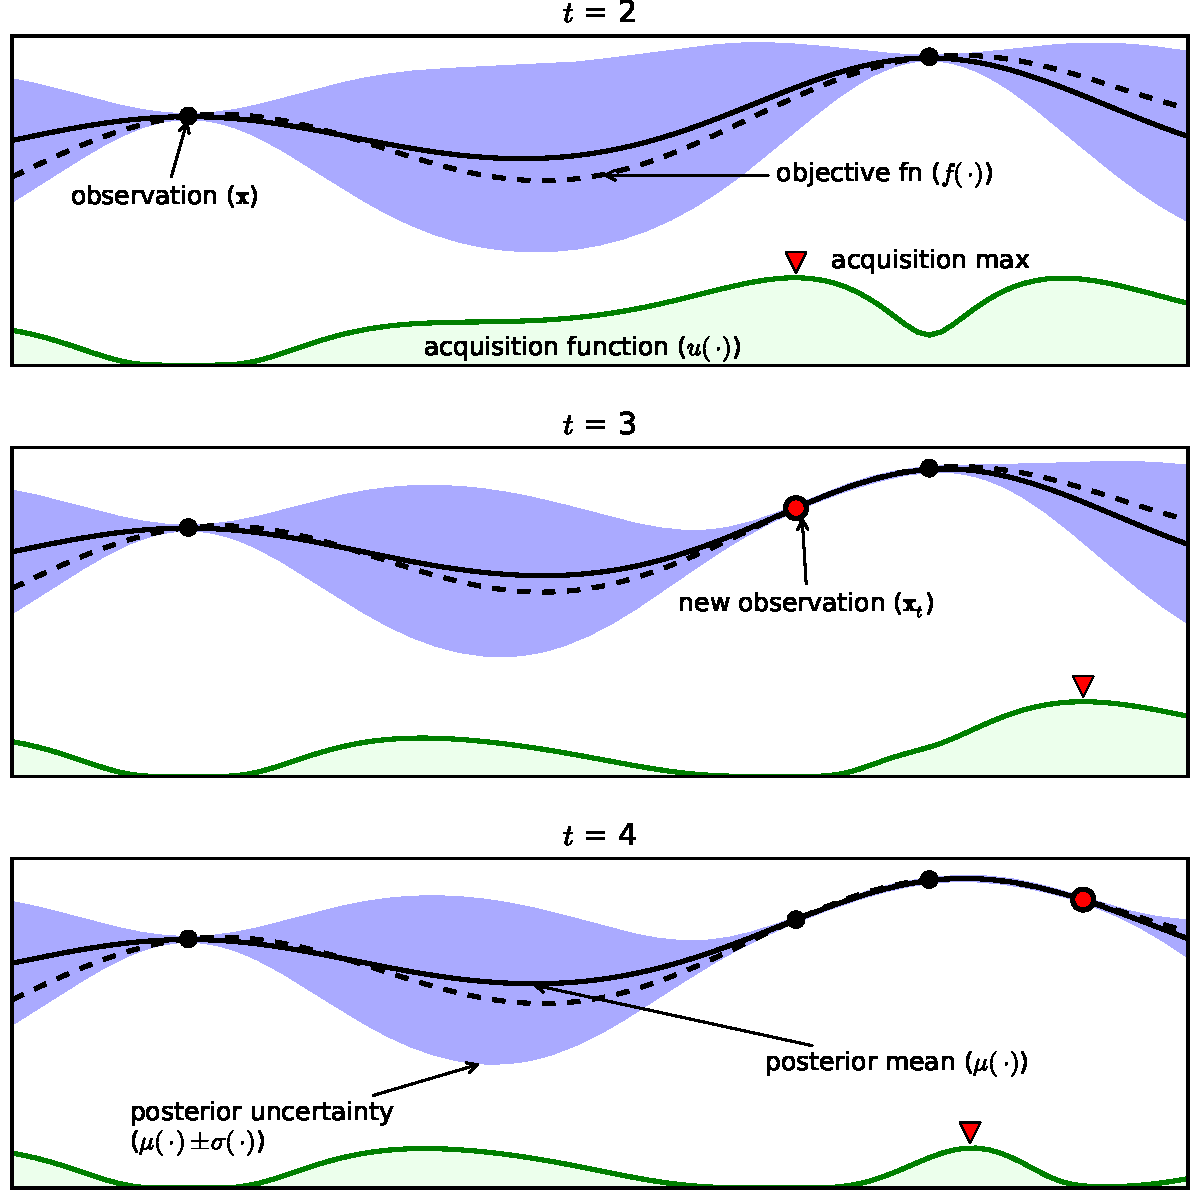
\includegraphics[width=0.85\textwidth]{figures/ml/toyGPtext3.pdf}
\caption{
Illustration of Bayesian optimization in a toy 1D problem \cite{Brochu2010}.
TODO
}
\label{fig:BO_ex}
\end{figure}

% TODO remember to read Brochu2010 section 5

%%%%%%%%%%%%%%%%%%%%%%%%%%%%%%%%%%%%%%%%%%%%%%%%%%%%%%%%
\subsection{Gaussian Mixture Model (GMM)}
\label{additional:unsupervised:GMM}
% TODO

%%%%%%%%%%%%%%%%%%%%%%%%%%%%%%%%%%%%%%%%%%%%%%%%%%%%%%%%
\subsection{\texorpdfstring{$\epsilon$}{epsilon}-Means}
\label{additional:unsupervised:epsilonMean}
% TODO

%%%%%%%%%%%%%%%%%%%%%%%%%%%%%%%%%%%%%%%%%%%%%%%%%%%%%%%%
\subsection{Louvain Method}
\label{additional:unsupervised:louvain}
% TODO

%%%%%%%%%%%%%%%%%%%%%%%%%%%%%%%%%%%%%%%%%%%%%%%%%%%%%%%%
\subsection{Variational Autoencoders (VAE)}
\label{additional:unsupervised:VAE}
% TODO

%%%%%%%%%%%%%%%%%%%%%%%%%%%%%%%%%%%%%%%%%%%%%%%%%%%%%%%%
\subsection{Support Vector Clustering}
\label{additional:unsupervised:SVC}
% TODO

